\section{Durchführung}
\label{sec:Durchführung}

Es werden die in Abbildung \ref{fig:bild1} und \ref{fig:bild2} abgebildeten Versuchsaufbauten verwendet.

\begin{figure}
    \centering
    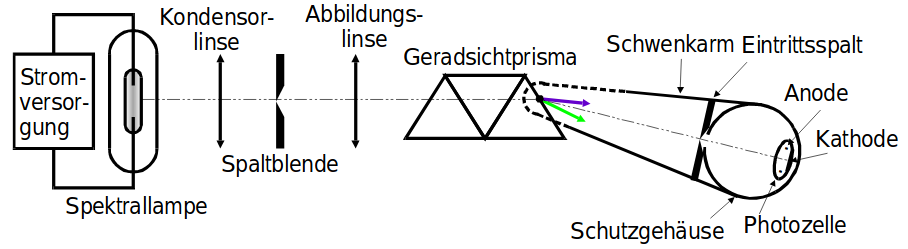
\includegraphics[scale=0.4]{content/bild2.png}
    \caption{Optischer Aufbau. [1]}
    \label{fig:bild2}
\end{figure}

Das Licht der Spektrallampe fällt, wie in Abbildung \ref{fig:bild2} dargestellt, durch
die Kondensatorlinse, eine Blende und die Abbildungslinse. Dabei wird das Licht gebündelt und ein
scharfes Bild erzeugt. Das Geradsichstprisma bricht die Spektrallinien verschiedener Frequenzen in 
verschiedenen Winkeln.
Durch Verstellung der Photozellenposition treffen die verschieden Spektrallinien in der Photozelle auf.

Der Photostrom $I_\lambda$ wird in Abhängigkeit von $U_\text{g}$ für verschiedene Lichtfrequenzen gemessen.
Für die Spektrallinie der Wellenlänge $\lambda = \SI{578}{\nano\meter}$ werden viele Messwerte im Messintervall
von $\SI{-20}{\volt} \leq U_\text{g} \leq \SI{20}{\volt}$ aufgenommen.
